\chapter{Protocolos de Sincronização de Simulação Distribuída}
%falar um pouco sobre sincronização%

\section{Protocolos Existentes}
\label{cap:protocolos}

Como foi discutido no capítulo anterior, com a necessidade da sincronização de processos que executam em ambientes diferentes, já que as máquinas tem seus próprios espaços de memória e relógios físicos, faz-se necessária a utilização de ferramentas para sincronizar o sistema. Para isto, os protocolos para a computação distribuída foram criados.

Este capítulo apresenta uma breve discussão dos protocolos conservativos e dos protocolos otimistas, além de apresentar o 

\section{Protocolos Conservativos}
\label{sec:protocons}

	Os primeiros autores a tratar os problemas de sincronização nos programas de simulação foram Chandy e Misra(1979) e Bryant(1977), assim batizado esse tipo de algorítmo de CMB em homenagem\cite{CMB1,CMB2}. Esse método trata os processos em uma linha de tempo cronológica, não deixando nenhum processo ocorrer fora de seu tempo de execução. Por sua vez, apresenta um problema quanto a determinar se é seguro ou não a execução de um processo, podendo provocar \textit{deadlock} no sistema.

		No CMB, os canais de comunicação entre os processos já são previamente especificados antes da simulação, ou seja, um processo só se comunicará com outro, caso um canal já tenha sido programado anteriormente.	Neste tipo de protocolo, como os canais de comunicação entre os processos são previamente conhecidos, é possível determinar o tempo lógico dos canais de comunicação entre os processos vizinhos, pois cada mensagem é rotulada de acordo com o \textit{local virtual time} (LVT) de sua máquina. 
	
Misra(1986) sugeriu um mecanismo para resolver o problema dos \textit{deadlocks} provocados por canais que possuem LVTs desatualizados. Seu mecanismo utiliza mensagens nulas para o cálculo do LVT. No entanto, isto pode causar a sobrecarga no sistema e lentidão na rede. Uma variação desta solução seria o envio de mensagens nulas sob demanda, com frequência dada por um temporizador ou quando houver canais com fila vazia.

	Há outros protocolos conservativos existentes: SRADS \cite{REYNOLDS82} , Appointments \cite{REYNOLDS84} , Turner Carrier-null Scheme \cite{CAITURNER} e SPaDES/Java\cite{TEONG} são alguns exemplos.


\section{Protocolos Otimistas}
\label{sec:protootimo}

O que difere basicamente um protocolo otimista de um conservativo, é o modo como ele trata os erros de causa e efeito. Enquanto os protocolos conservativos previnem esses erros, os protocolos otimistas permitem que essa regra seja violada, provendo mecanismos para retornar (\textit{rollback}) a simulação e reconstruí-la de forma consistente.  

Assim como nos protocolos conservativos, os processos nos protocolos otimistas se intercomunicam através de mensagens, uma vez que estes não possuem dados compartilhados entre si. Porém, diferente dos protocolos conservativos, nos protocolos otimistas não existe uma garantia que uma mensagem vai ser entregue na mesma ordem em que foi enviada, e também não há como garantir que uma mensagem não seja recebida com um \textit{timestamp} menor que o LVT daquele processo.

Quando uma mensagem chega à um processo com um tempo inferior ao seu LVT, ela é denominada  \textit{straggler}. Quando uma mensagem \textit{straggler} surge, a situação  é tratada com um \textit{rollback}. Este, por sua vez, deve ser capaz de restaurar a computação, retornando o processamento para um estado global consistente, para poder processar a mensagem e dar continuidade à simulação.

	
\section{Time Warp}
	Um dos mais conhecidos protocolos otimistas é o Time Warp, que possui algumas implementações, tais como \textit{Jade Time Warp} \cite{BAEZNER1}, o sistema \textit{SPEE-DES} (\textit{Synchronous Parallel Environment for Emulation and Discrete Event Simulation})\cite{STEINMAN92}, o \textit{WARPED} \cite{WARPED} e o \textit{Georgia Tech Time Warp (GTW)} \cite{DAS94}. O \textit{Time Warp} foi originalmente proposto por Jefferson(1985). 

O \textit{Time Warp} pode ser dividido em duas partes distintas: o controle local, interno a cada processo, o qual é responsável por garantir que a execução dos eventos seja feita em ordem cronológica dentro de cada processo; e o controle global, destinado ao gerenciamento de memória e ao cálculo do \textit{Global Virtual Time}(GVT)(JEFERSON, 1985).

O comportamento da simulação no protocolo \textit{Time Warp} é semelhante ao de um programa sequêncial. Os eventos internos à um processo são organizados em uma lista, respeitando os seus \textit{timestamps}. Estes eventos são retirados da lista para serem tratados. 

A comunicação entre os processos é feita através de troca de mensagens. As mensagens, assim como os eventos, também são rotuladas com uma marca de tempo. 

Os eventos processados podem gerar mensagens a serem enviadas a outros processos. Estas mensagens, por sua vez, geram eventos que devem ser alocados na lista de eventos futuros para serem tratados, respeitando o seu \textit{timestamp}.

Uma vez que um processo recebe uma mensagem com um \textit{timestamp} inferior ao valor do seu LVT, tem-se uma situação de inconsistência no sistema. Como um protocolo otimista, o \textit{Time Warp} deve ser capaz de retornar a simulação a fim de reconstruí-la, agora considerando também a mensagem que havia chegado fora da ordem.
	
No exemplo da figura~\ref{fig:strangler}, o evento $e_{1}^{2}$ envia uma mensagem com LVT igual a 2 para um processo que já está no tempo 3. Isso gera uma mensagem \textit{straggler}, pois o evento $e_{3}^{3}$ só deveria ser executado após o recebimento da mensagem. Para a correção, o protocolo deve garantir que o evento $e_{3}^{3}$ seja desfeito e que ele somente seja executado depois do tratamento da mensagem enviada pelo evento $e_{1}^{2}$.

\begin{figure}
  \centerline{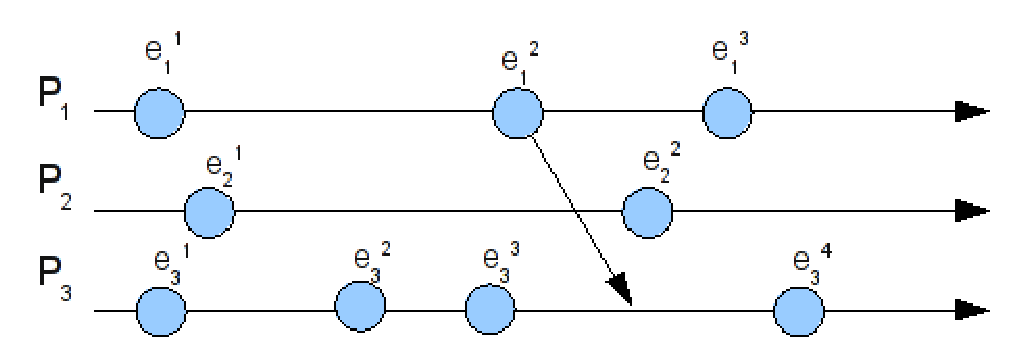
\includegraphics[scale=0.6]{strangler.eps}}
  \caption{Mensagem strangler.}
\label{fig:strangler}
\end{figure}

\subsection{\textit{Rollback} primário e \textit{Rollback} secundário}
Assim que uma mensagem \textit{straggler} é identificada por um processo, este retorna a um tempo lógico imediatamente inferior ao \textit{timestamp} da mensagem recebida. Isto é feito para que os dados provenientes da mensagem sejam tratados, mantendo a ordem natural de execução da simulação.

Porém, um processo que necessitou fazer um \textit{rollback} pode ter enviado mensagens a outros processos em um tempo superior ao seu tempo lógico de retorno. Todas essas mensagens enviadas devem ser desconsideradas pelo sistema, e os processos que porventura tenham tratado eventos gerados por estas mensagens devem também retornar, podendo gerar novos \textit{rollbacks} no sistema.

Um \textit{rollback} que foi gerado devido ao recebimento de uma mensagem \textit{straggler} é chamado de \textit{rollback} primário, já um retorno causado por efeito de um outro \textit{rollback} é chamado de \textit{rollback} secundário.

\subsection{Anti-Mensagem}
Ao realizar um \textit{rollback}, um processo deve verificar se foram enviadas mensagens com tempo lógico superior ao valor do seu tempo de retorno. Para toda mensagem enviada, o processo deve mandar uma anti-mensagem, indicando que as mensagens anteriores devem ser desconsideradas.

Ao receber uma anti-mensagem, um processo pode encontrar três situações distintas:
\begin{itemize}
	\item O evento gerado pela mensagem a ser cancelada já foi tratado. Então deve-se realizar um retorno (\textit{rollback} secundário) para um tempo lógico inferior ao recebimento da mensagem, e fazer, se necessário, também o envio de anti-mensagens;

	\item O evento gerado ainda está na fila a espera da execução. Neste caso o processo apenas exclui este evento da lista de eventos futuros;

	\item Anti-mensagem chegar ao processo antes da mensagem. Caso essa situação aconteça, o processo armazena a anti-mensagem para, quando a mensagem chegar, eliminar as duas.
\end{itemize}

\section{\textit{RollBack} Solidário}

	Assim como o \textit{Time Warp}, o \textit{Rollback} Solidário é um protocolo otimista, entretanto, ele apresenta diferenças significativas na maneira com que os retornos são realizados para sincronizar os processos durante a simulação distribuída.
	
	Uma primeira diferença que pode ser citada é que no protocolo \textit{Rollback} Solidário, quando um erro de causa e efeito é identificado durante a simulação, todos os processos executam em conjunto um \textit{rollback} para um \textit{checkpoint} global consistente, enquanto no protocolo \textit{Time Warp}, em um primeiro instante, apenas o processo que identificou o erro de causa e efeito realiza o \textit{rollback}.

	\textit{Checkpoints} são estados de um processo armazenados em um mecanismo "persistente" de memória para a recuperação de um sistema em caso de falhas\cite{EDMARMO}. Um checkpoint local é o conjunto de dados de um processo num determinado tempo da simulação e um \textit{checkpoint} global é um conjunto de \textit{checkpoints} locais, sendo um para cada processo da simulação.

	Para que um \textit{checkpint} global possa ser utilizado como um ponto de retorno no caso de um erro na simulação, deve-se garantir que esse checkpoint global seja consistente. Para ser considerado consistente, um \textit{checkpoint} global deve estar associado a um corte global consistente e nenhum \textit{checkpoint} do conjunto deve possuir relação de dependência com outro \textit{checkpoint} do mesmo conjunto.
	
	Estas diferença na maneira de se realizar o retorno dos procesos dispensa a necessidade de se enviar anti-mensagens, que poderiam provocar \textit{rollbacks} em outros processos, evitando assim a ocorrência de \textit{rollback} em cascata.

\section{O comportamento geral do protocolo \textit{Rollback} Solidário}
	No decorrer de uma simulação, utilizando o protocolo \textit{Rollback} Solidário, assim como no \textit{Time warp}, os processos se intercomunicam através de mensagens. Porém, ao identificar um erro de causa e efeito, ou seja, ao se receber uma mensagem \textit{straggler}, o sistema se comporta da seguinte forma:

\begin{itemize}
	\item O processo que recebeu a mensagem \textit{straggler} identifica o estado salvo (\textit{checkpoint}) com tempo lógico imediatamente anterior ao \textit{timestamp} da mensagem.
	\item O sistema se encarrega de selecionar o \textit{checkpoint} global consistente que contenha este estado identificado e que cause a menor sobrecarga durante o  \textit{rollback} (mínimo possível de eventos para se retornar).
	\item Toda a simulação realiza o retorno à este \textit{checkpoint} global consistente de maneira uniforme.
\end{itemize}

\section{Recuperação dos Estados Durante um \textit{Rollback}}
A eficiência do protocolo \textit{Rollback} Solidário está diretamente ligada em como ele retorna à um \textit{checkpoint} global consistente após identificar uma inconsistência na simulação. O \textit{checkpoint} global consistente a ser selecionado deve gerar o menor custo para o sistema. Para isto, deve-se garantir que os processos voltem a menor distância possível necessária para recompôr o processamento.

	Considerando o exemplo da figura~\ref{fig:linhasrec}, sabe-se que em relação a seus tempos lógicos  tem-se $t''<b'<t'<t$. Assim sendo, supondo que o processo $p_{1}$ receba uma mensagem no tempo $t$, gerando um evento que deveria ter sido executada no tempo $t'$, ocorre que neste momento o sistema deve retornar ao último \textit{checkpoint} global consistente que contenha o processo $b'$, que neste caso é o corte B. Porém, supondo que o processo $P_1$ recebe, no tempo $t$, uma mensagem que gera um evento a ser processado no tempo $t''$, anterior ao evento $b'$ , não pode-se admitir o corte B como linha de recuperação, devido ao tempo lógico de $b'$ ser maior que o tempo lógico de $t''$. Acontece aí então um \textit{rollback} para a linha de recuperação A. 
	
	Nota-se, nessa situação, que nem todos os processos precisam voltar para a mesma linha de recuperação. No exemplo da figura~\ref{fig:linhasrec}, tanto os processos P2 e P3 podem permanecer com os mesmos \textit{checkpoints} do corte B, uma vez que não houve troca de mensagens por parte dos processos entre os cortes A e B.
	
	Para garantir a eficiência do protocolo, deve-se garantir que a linha de recuperação preserve ao máximo os eventos já processados. Para isso, é necessário armazenar várias linhas de recuperação que passem por um mesmo \textit{checkpoint}.

\begin{figure}[htb]
  \centerline{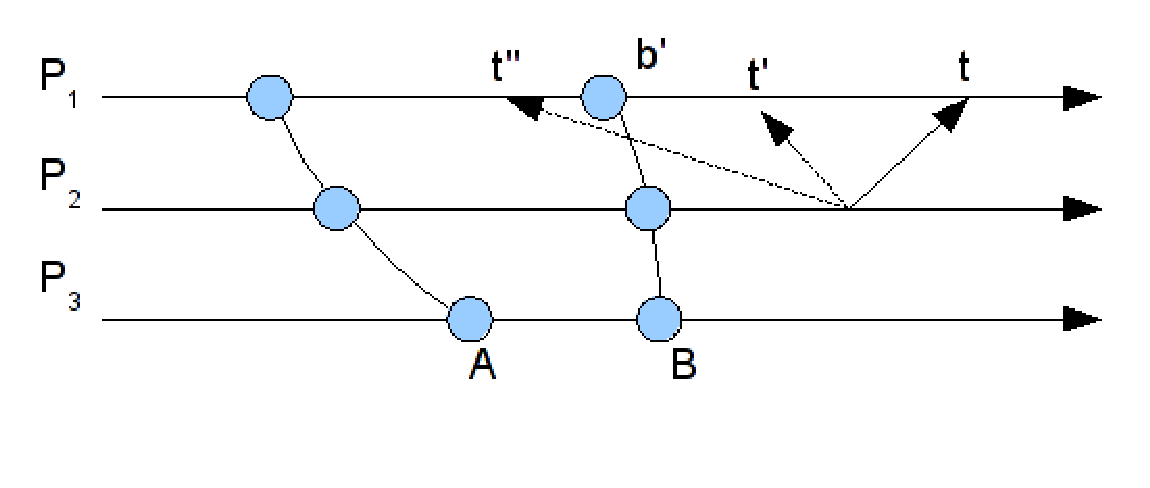
\includegraphics[scale=0.6]{cortes_rollback.eps}}
  \caption{Linhas de recuperação.}
\label{fig:linhasrec}
\end{figure}	


\section{Uma abordagem utilizando \textit{checkpoints} síncronos}
	Mecanismos de \textit{checkpoints} síncronos são mecanismos que exigem que os processos realizem seus checkpoints em conjunto para a obtenção de um \textit{checkpoint} global consistentes.	 Para o protocolo \textit{Rollback} Solidário utilizando \textit{checkpoints} síncronos são apresentadas as extenções dos os algorítimos \textit{Sync-and-Stop}\cite{Plank93}  e \textit{Chandy-Lamport}\cite{ChandyLamport}.


\section{Rollback Solidário utilizando mecanismos de \textit{checkpoints} Semi-Síncronos}

	Para a construção da linha de recuperação na abordagem semi-síncrona, um processo, denominado processo observador, fica encarregado de receber os vetores de dependência associados aos respectivos \textit{checkpoints} de cada processo e identificar o \textit{checkpoint} global consistente para onde a simulação deve retornar.

	Ao realizar um \textit{checkpoint}, um processo envia ao observador um vetor com as suas dependências. Com isto, o processo observador constrói um matriz quadrada $M$ de ordem $n$, onde $n$ é o número de processos da simulação. Cada linha $i$ da matriz é o vetor de dependência de um processo $p_i$, que contém as informações de dependência do último \textit{checkpoint} realizado por esse processo $p_i$. 

	A matriz é iniciada com o primeiro \textit{checkpoint} de cada processo. Como todos os processos no início da simulação estão num mesmo evento inicial, a matriz $M$ é iniciada como uma matriz identidade.

	A diagonal principal da matriz $M$ poderá indicar uma linha de recuperação da simulação. Para que esta linha de recuperação seja válida, todos os elementos de uma coluna que não fizerem parte da diagonal principal da matriz devem possuir valores menores do que o elemento pertencente à diagonal.  

	Para garantir que todas as possíveis linhas de recuperação sejam identificados um novo vetor de dependência é recebido pelo processo observador, o último vetor referente ao processo que realizou o \textit{checkpoint} não deve ser descartado, mas sim armazenado para futuras consultas.

	A solução para se armazenar os diversos vetores está em utilizar, ao invés de matriz quadrada uma lista encadeada para cada processo, cada uma contendo os vetores de dependência.

	Ao receber um aviso de \textit{rollback}, proveniente de algum processo, cabe ao processo observador percorrer as listas e identificar os \textit{checkpoints} adequados para constituir a linha de recuperação correspondente.
	
	


